\chapter{Wireless Networks}
Wireless Networks are composed of \textbf{hosts}, which are end-system devices that run
applications, typically battery powered.
\note{Recall that \ul{\textit{wireless} $\neq$ \textit{mobility}}}

In general Wireless Networks may be based on the interaction \textit{hosts} $\longrightarrow$ \textit{base station} ---or access point--- or \textit{hosts} $\longrightarrow$ \textit{hosts}.
The two resulting functioning modes are called \textit{Infrastructure} and \textit{Ad hoc networking}.

\begin{paracol}{2}
   \colfill
   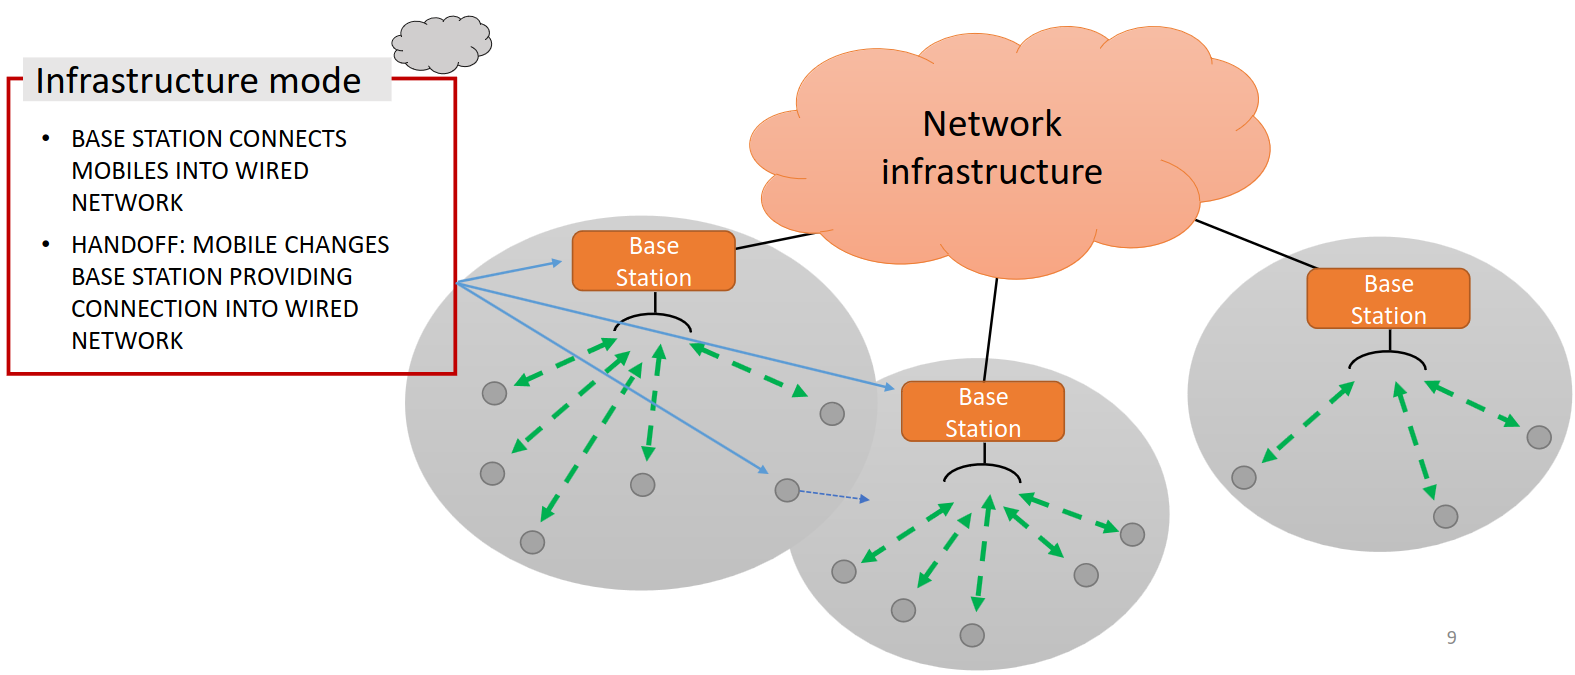
\includegraphics[width=0.9\columnwidth]{images/wirelessnet_infrastructure.png}
   \colfill
   \switchcolumn
   \colfill
   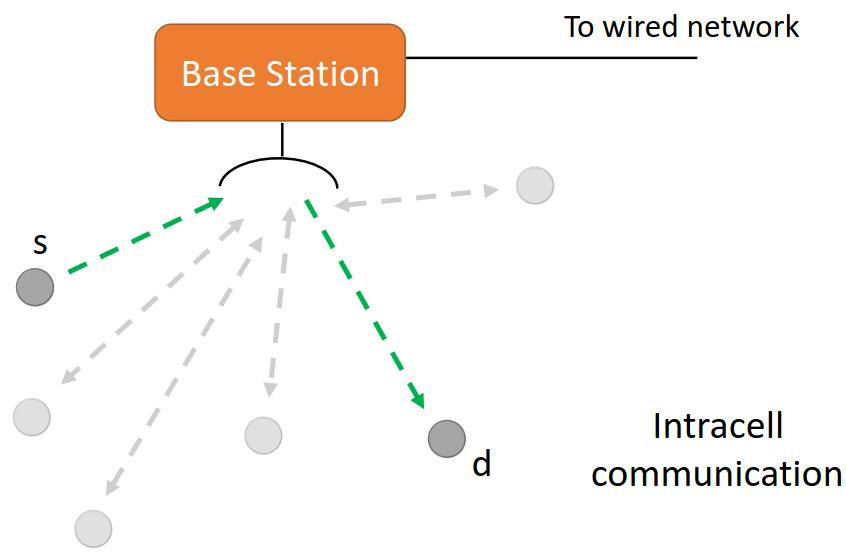
\includegraphics[width=0.9\columnwidth]{images/wirelessnet_cell1.png}\\
   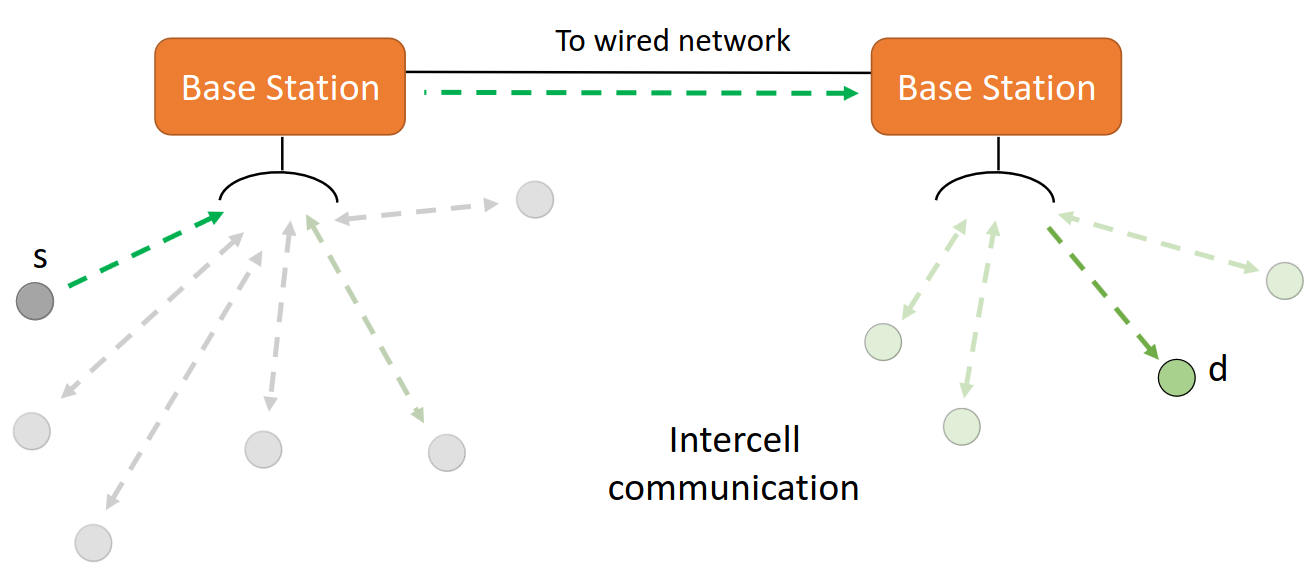
\includegraphics[width=0.9\columnwidth]{images/wirelessnet_cell2.png}
   \colfill
\end{paracol}

\begin{figure}[htbp]
   \centering
   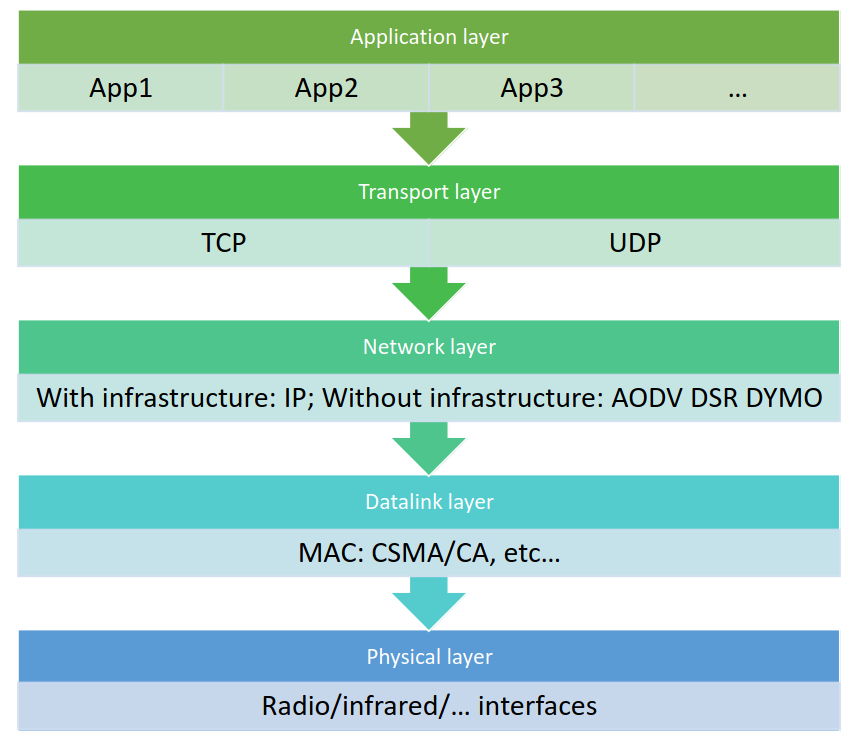
\includegraphics{images/stack.png}
   \caption{Protocol stack}
   \label{fig:stack}
\end{figure}

\section{Link Layer}
\subsection{CSMA/CD}
Basic idea of CSMA/CD:
\begin{enumerate}
   \item When a station has a frame to send it listens to
   the channel to see if anyone else is transmitting
   \item if the channel is busy, the station waits until it
   becomes idle
   \item when channel is idle, the station transmits the
   frame
   \item if a collision occurs the station waits a random
   amount of time and repeats the procedure.
   \item[]\note{Refer to the slides of 21 February for more in depth usage examples}
\end{enumerate}

In short: \ul{CSMA/CD performs poorly in wireless networks}.
Firstly because CSMA/CD detects collisions while transmitting, which is ok for wired networks, but not for wireless ones.
Secondarily, what truly matters is the interference at the \textit{receiver}, \textbf{not} at the \textit{sender}, causing the two problems known as \textit{\ul{hidden}} and \ul{\textit{exposed terminal}} problems;
to better understand this point, look at the following figure, consider that at the sender, the signal strength of its own transmission (self-signal) would be too strong to detect a collision by another transmitter, making collisions happen at the receiver.

\begin{figure}[htbp]
   \centering
   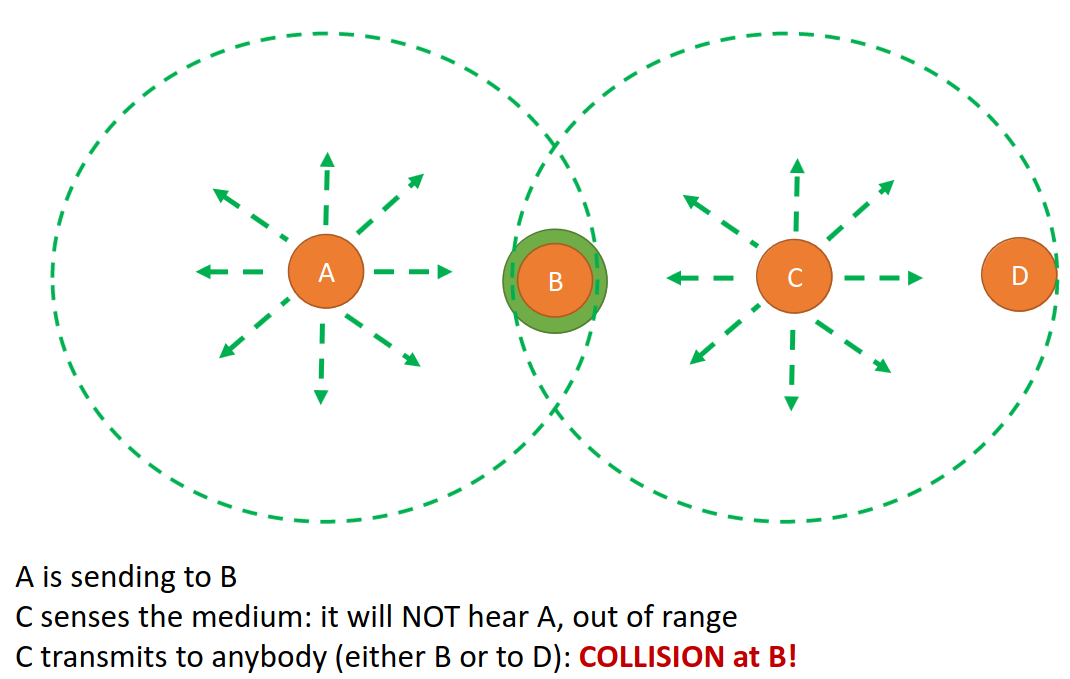
\includegraphics{images/hiddenterminal.png}
   \caption{\textbf{Hidden Terminal} problem}
   \textit{Two or more stations which are out of range of each other transmit simultaneously to a common
   recipient}
   \label{fig:hiddenterminal}
\end{figure}


\begin{figure}[htbp]
   \centering
   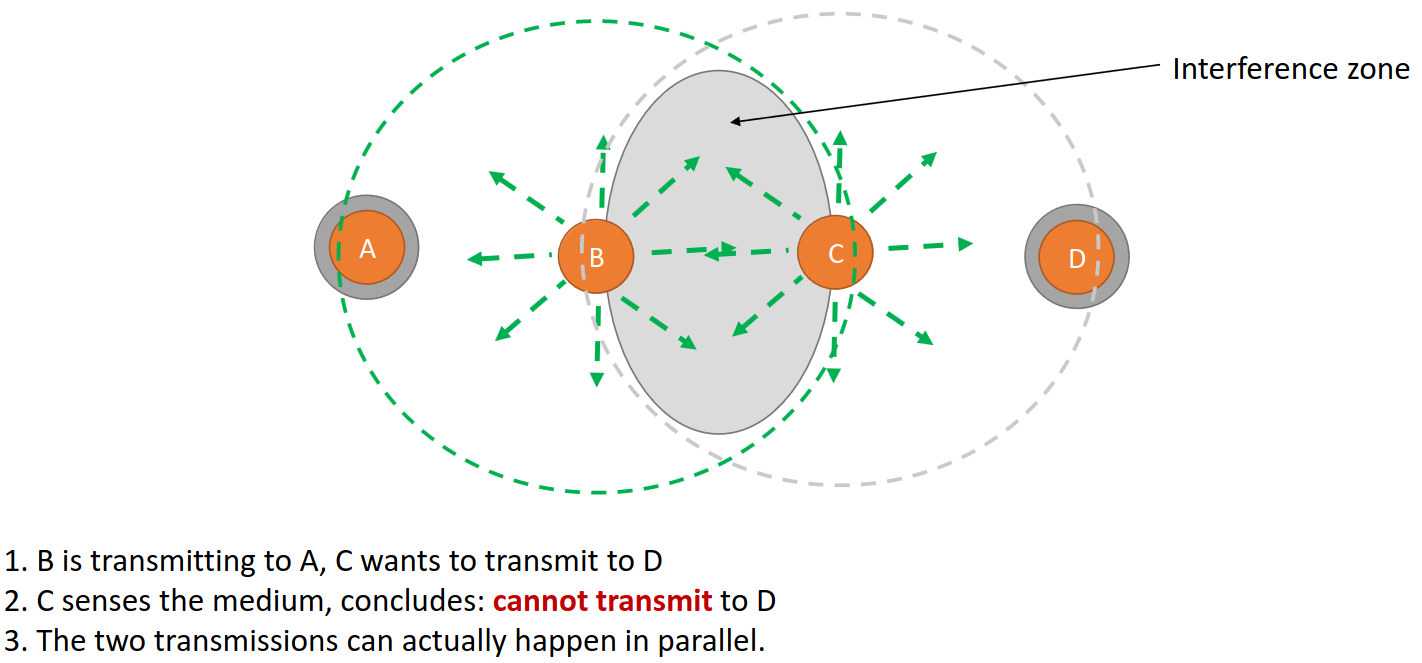
\includegraphics{images/exposedterminal.png}
   \caption{\textbf{Exposed Terminal} problem}
   \textit{A transmitting station is prevented from sending frames due to interference with another
   transmitting station}
   \label{fig:exposedterminal}
\end{figure}

\newpage
\subsection{MACA}
\begin{figure}[htbp]
   \centering
   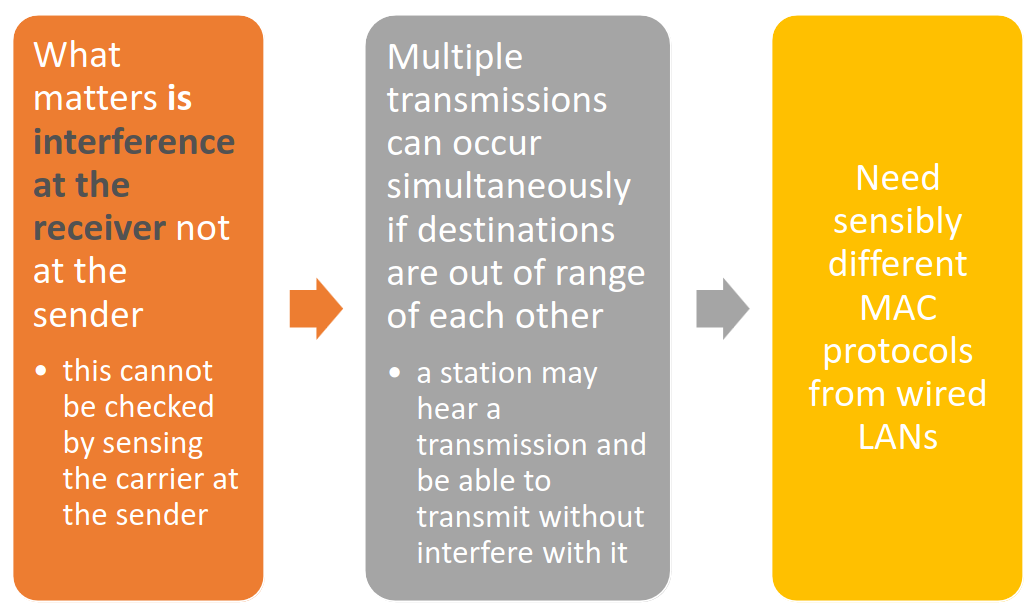
\includegraphics{images/MACA_motivations.png}
   \caption{MACA Motivations}
   \label{fig:MACA_motivations}
\end{figure}

\textbf{MACA} stands for \textit{Multiple Access with Collision Avoidance}
\begin{enumerate}
   \item stimulate the receiver into transmitting a short
   frame first
   \item then transmit a (long) data frame
   \item stations hearing the short frame refrain from
   transmitting during the transmission of the
   subsequent data frame
\end{enumerate}

Basically, a transmitting node sends a \textit{Request to Send} \texttt{RTS} and a receiving node answers with \textit{Clear to Send} \texttt{CTS}.
Other nodes which hear \texttt{CTS} \ul{must stay silent until the transmission is over}.
Hearing \texttt{RTS} instead does not imply to stay silent, i.e. hearing a \texttt{RTS} does not forbid to transmit stuff to other nodes.

\note{\ul{Further details and examples on how the protocol works are on the slides.}}
\nl

\textbf{MACAW} implements some improvements to MACA:
\begin{itemize}
   \item ACK frame to acknowledge a
   successful data frame
   \item added Carrier Sensing to keep a station from
   transmitting RTS when a nearby station is also
   transmitting an RTS to the same destination
   \item mechanisms to exchange information among
   stations and recognize temporary congestion
   problems
   \item[] \note{CSMA/CA used in IEEE 802.11 is based on MACAW}
\end{itemize}